% Options for packages loaded elsewhere
\PassOptionsToPackage{unicode}{hyperref}
\PassOptionsToPackage{hyphens}{url}
\documentclass[
]{article}
\usepackage{xcolor}
\usepackage{amsmath,amssymb}
\setcounter{secnumdepth}{-\maxdimen} % remove section numbering
\usepackage{iftex}
\ifPDFTeX
  \usepackage[T1]{fontenc}
  \usepackage[utf8]{inputenc}
  \usepackage{textcomp} % provide euro and other symbols
\else % if luatex or xetex
  \usepackage{unicode-math} % this also loads fontspec
  \defaultfontfeatures{Scale=MatchLowercase}
  \defaultfontfeatures[\rmfamily]{Ligatures=TeX,Scale=1}
\fi
\usepackage{lmodern}
\ifPDFTeX\else
  % xetex/luatex font selection
\fi
% Use upquote if available, for straight quotes in verbatim environments
\IfFileExists{upquote.sty}{\usepackage{upquote}}{}
\IfFileExists{microtype.sty}{% use microtype if available
  \usepackage[]{microtype}
  \UseMicrotypeSet[protrusion]{basicmath} % disable protrusion for tt fonts
}{}
\makeatletter
\@ifundefined{KOMAClassName}{% if non-KOMA class
  \IfFileExists{parskip.sty}{%
    \usepackage{parskip}
  }{% else
    \setlength{\parindent}{0pt}
    \setlength{\parskip}{6pt plus 2pt minus 1pt}}
}{% if KOMA class
  \KOMAoptions{parskip=half}}
\makeatother
\usepackage{longtable,booktabs,array}
\newcounter{none} % for unnumbered tables
\usepackage{calc} % for calculating minipage widths
% Correct order of tables after \paragraph or \subparagraph
\usepackage{etoolbox}
\makeatletter
\patchcmd\longtable{\par}{\if@noskipsec\mbox{}\fi\par}{}{}
\makeatother
% Allow footnotes in longtable head/foot
\IfFileExists{footnotehyper.sty}{\usepackage{footnotehyper}}{\usepackage{footnote}}
\makesavenoteenv{longtable}
\usepackage{graphicx}
\makeatletter
\newsavebox\pandoc@box
\newcommand*\pandocbounded[1]{% scales image to fit in text height/width
  \sbox\pandoc@box{#1}%
  \Gscale@div\@tempa{\textheight}{\dimexpr\ht\pandoc@box+\dp\pandoc@box\relax}%
  \Gscale@div\@tempb{\linewidth}{\wd\pandoc@box}%
  \ifdim\@tempb\p@<\@tempa\p@\let\@tempa\@tempb\fi% select the smaller of both
  \ifdim\@tempa\p@<\p@\scalebox{\@tempa}{\usebox\pandoc@box}%
  \else\usebox{\pandoc@box}%
  \fi%
}
% Set default figure placement to htbp
\def\fps@figure{htbp}
\makeatother
\setlength{\emergencystretch}{3em} % prevent overfull lines
\providecommand{\tightlist}{%
  \setlength{\itemsep}{0pt}\setlength{\parskip}{0pt}}
\usepackage{bookmark}
\IfFileExists{xurl.sty}{\usepackage{xurl}}{} % add URL line breaks if available
\urlstyle{same}
\hypersetup{
  pdftitle={Overton Framework Companion Note v0.1: The Micro-Coercion of Speed},
  pdfauthor={K Overton},
  pdfkeywords={protective computing, software architecture, artificial
intelligence, cognitive load, system integrity, Overton Framework},
  hidelinks,
  pdfcreator={LaTeX via pandoc}}

\title{Overton Framework Companion Note v0.1: The Micro-Coercion of
Speed}
\author{K Overton}
\date{March 2026}

\begin{document}
\maketitle

\section{Overton Framework Companion Note v0.1: The Micro-Coercion of
Speed}\label{overton-framework-companion-note-v01-the-micro-coercion-of-speed}

\textbf{Why friction is an engineering prerequisite in AI-assisted
development systems}

\textbf{Author:} K Overton\\
\textbf{Date:} March 2026\\
\textbf{Version:} 0.1.0-preprint\\
\textbf{License:} Creative Commons Attribution 4.0 International
(CC-BY-4.0)

\begin{center}\rule{0.5\linewidth}{0.5pt}\end{center}

\section{Abstract}\label{abstract}

AI-assisted development environments compress generation time while
leaving verification cost largely unchanged. This asymmetry creates a
recurrent operational hazard: under velocity pressure, developers
increasingly accept plausible outputs without sufficient validation.

We define this effect as the \textbf{micro-coercion of speed}: a
system-level pressure gradient that shifts the burden-of-proof from tool
output to human rebuttal.

This paper proposes a control orientation for Protective Computing
contexts: the engineering of \textbf{cognitive interlocks} that force
verification before integration in high-impact paths.

Three implementation classes are defined:

\begin{itemize}
\tightlist
\item
  IDE boundary interlocks
\item
  generation-verification separation
\item
  cognitive slow paths
\end{itemize}

These controls restore system integrity by constraining the interaction
between AI generation velocity and human verification limits.

\begin{center}\rule{0.5\linewidth}{0.5pt}\end{center}

\section{1. Introduction and Problem
Statement}\label{1-introduction-and-problem-statement}

AI coding systems optimize \textbf{generation throughput}.

Systemic integrity, however, depends on \textbf{verification
throughput}.

When generation throughput exceeds verification capacity, latent defects
accumulate behind an appearance of productivity.

The resulting failure pattern is not purely technical.

It is \textbf{cognitive and procedural}.

Current toolchains accelerate proposal creation disproportionately
relative to correctness establishment.

\begin{center}\rule{0.5\linewidth}{0.5pt}\end{center}

\subsection{1.1 Burden-of-Proof
Inversion}\label{11-burden-of-proof-inversion}

Polished machine output is cognitively treated as \textbf{presumptively
correct} under velocity pressure.

This inverts the architectural burden of proof.

\textbf{Expected baseline (Safe)}\\
Output must earn trust through verifiable constraints.

\textbf{Observed baseline (Unsafe)}\\
The reviewer must actively disprove the output.

This inversion dramatically increases the probability that defects pass
into production.

\begin{center}\rule{0.5\linewidth}{0.5pt}\end{center}

\subsection{1.2 Deferred Failure
Behavior}\label{12-deferred-failure-behavior}

Unverified velocity frequently appears successful until systems
encounter stressors:

\begin{itemize}
\tightlist
\item
  unusual input
\item
  system scale
\item
  operational fatigue
\item
  incident conditions
\end{itemize}

Failures emerge \textbf{downstream}, far from the original generation
event.

\begin{center}\rule{0.5\linewidth}{0.5pt}\end{center}

\section{2. Theoretical Framework: Physical vs Cognitive
Interlocks}\label{2-theoretical-framework-physical-vs-cognitive-interlocks}

Safety-critical physical systems assume imperfect operators.

They embed \textbf{interlocks} that prevent hazardous shortcuts.

Examples include:

\begin{itemize}
\tightlist
\item
  OSHA lockout/tagout procedures
\item
  pressure safety switches
\item
  thermal cutoffs
\item
  keyed disconnects
\end{itemize}

These mechanisms do not eliminate speed pressure.

They \textbf{bound it}.

\begin{center}\rule{0.5\linewidth}{0.5pt}\end{center}

\subsection{Transferable Design
Pattern}\label{transferable-design-pattern}

The pattern translates directly to software architecture.

{\def\LTcaptype{none} % do not increment counter
\begin{longtable}[]{@{}lll@{}}
\toprule\noalign{}
Domain & Interlock Type & Effect \\
\midrule\noalign{}
\endhead
\bottomrule\noalign{}
\endlastfoot
Physical engineering & Mechanical interlock & Prevent unsafe states \\
Software systems & Cognitive interlock & Prevent unverified
integration \\
\end{longtable}
}

In both domains, \textbf{safety emerges from design constraints rather
than operator perfection}.

\begin{center}\rule{0.5\linewidth}{0.5pt}\end{center}

\section{3. Architectural Control
Model}\label{3-architectural-control-model}

\subsection{3.1 Risk Pathway}\label{31-risk-pathway}

\pandocbounded{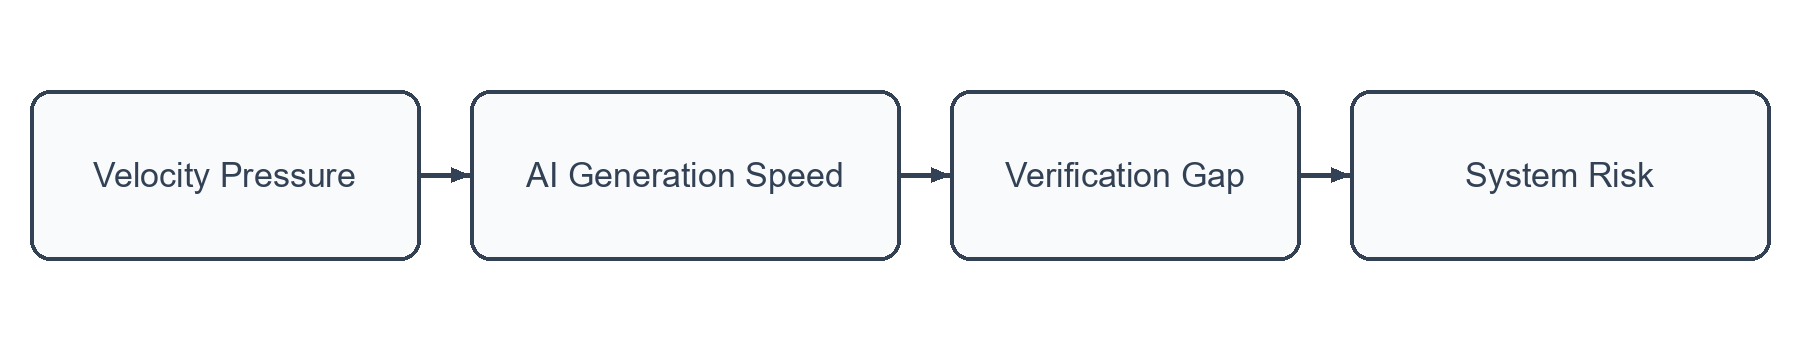
\includegraphics[keepaspectratio,alt={Risk Pathway}]{figures/risk-pathway.png}}

\begin{center}\rule{0.5\linewidth}{0.5pt}\end{center}

\subsection{3.2 Protective Pathway}\label{32-protective-pathway}

The Overton Framework introduces \textbf{cognitive interlocks} to
interrupt this pipeline.

\pandocbounded{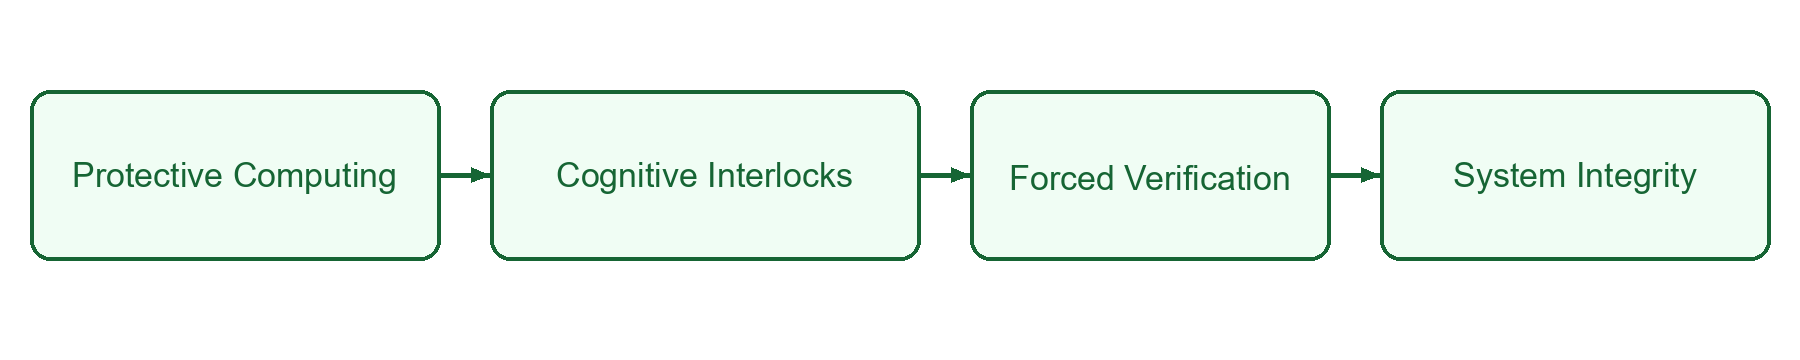
\includegraphics[keepaspectratio,alt={Protective Pathway}]{figures/protective-pathway.png}}

\begin{center}\rule{0.5\linewidth}{0.5pt}\end{center}

\subsection{3.3 Control Classes}\label{33-control-classes}

\subsubsection{1. IDE Boundary
Interlocks}\label{1-ide-boundary-interlocks}

Enforce safety boundaries at the authoring environment level.

Examples:

\begin{itemize}
\tightlist
\item
  mandatory query parameterization
\item
  sensitive API call constraints
\item
  build failures on unsafe patterns
\end{itemize}

These controls eliminate reliance on reviewer recall.

\begin{center}\rule{0.5\linewidth}{0.5pt}\end{center}

\subsubsection{2. Generation-Verification
Separation}\label{2-generation-verification-separation}

Treat AI output as \textbf{draft state} rather than trusted logic.

Integration into protected paths requires explicit human checkpoints.

\begin{center}\rule{0.5\linewidth}{0.5pt}\end{center}

\subsubsection{3. Cognitive Slow Paths}\label{3-cognitive-slow-paths}

Introduce friction deliberately when high-impact logic is modified.

Examples include:

\begin{itemize}
\tightlist
\item
  generated-diff emphasis
\item
  mandatory rationale fields
\item
  sensitive-flow highlighting
\end{itemize}

These mechanisms shift the developer from \textbf{fast intuition to
deliberate reasoning}.

\begin{center}\rule{0.5\linewidth}{0.5pt}\end{center}

\section{4. Implementation
Guidelines}\label{4-implementation-guidelines}

\subsection{4.1 Minimal Adoption
Baseline}\label{41-minimal-adoption-baseline}

Systems implementing this model must:

\begin{enumerate}
\def\labelenumi{\arabic{enumi}.}
\tightlist
\item
  Mark generated hunks in code review metadata
\item
  Require reviewer rationale for changes touching sensitive boundaries
\item
  Block merges when verification evidence is absent
\end{enumerate}

\begin{center}\rule{0.5\linewidth}{0.5pt}\end{center}

\subsection{4.2 Expected Outcomes}\label{42-expected-outcomes}

Adoption produces measurable effects:

\begin{itemize}
\tightlist
\item
  reduced silent acceptance of generated logic
\item
  improved traceability for high-impact changes
\item
  stronger operator ownership under deadline pressure
\end{itemize}

\begin{center}\rule{0.5\linewidth}{0.5pt}\end{center}

\subsection{4.3 Trade-off Statement}\label{43-trade-off-statement}

These controls intentionally add \textbf{bounded friction}.

The objective is \textbf{not reduced development velocity}.

The objective is \textbf{reduced defect transfer from generation to
production under cognitive load}.

\begin{center}\rule{0.5\linewidth}{0.5pt}\end{center}

\section{5. Governance and Framework
Integration}\label{5-governance-and-framework-integration}

\subsection{5.1 Status}\label{51-status}

\begin{itemize}
\tightlist
\item
  \textbf{Document class:} Companion Note (non-canonical guidance)
\item
  \textbf{Intended role:} Bridge artifact from public narrative to
  formal architectural controls
\item
  \textbf{Canon relationship:} Interprets but does not supersede Overton
  Framework Canon requirements
\end{itemize}

\begin{center}\rule{0.5\linewidth}{0.5pt}\end{center}

\section{6. Velocity Pressure: Formal
Metric}\label{6-velocity-pressure-formal-metric}

\subsection{6.1 Definition}\label{61-definition}

Velocity Pressure (\(P_v\)) quantifies the ratio between AI generation
rate and human verification capacity.

\[
P_v = \frac{R_g}{C_v}
\]

Where:

\begin{itemize}
\tightlist
\item
  \(P_v\) = Velocity Pressure
\item
  \(R_g\) = Rate of AI-assisted code generation
\item
  \(C_v\) = Human cognitive verification capacity
\end{itemize}

\begin{center}\rule{0.5\linewidth}{0.5pt}\end{center}

\subsection{6.2 Interpretation}\label{62-interpretation}

{\def\LTcaptype{none} % do not increment counter
\begin{longtable}[]{@{}ll@{}}
\toprule\noalign{}
Condition & Meaning \\
\midrule\noalign{}
\endhead
\bottomrule\noalign{}
\endlastfoot
\(P_v \le 1\) & Verification capacity keeps pace with generation \\
\(P_v > 1\) & Verification gap forms \\
\(P_v \gg 1\) & Micro-coercion conditions likely \\
\end{longtable}
}

\begin{center}\rule{0.5\linewidth}{0.5pt}\end{center}

\subsection{6.3 Measurement
Methodology}\label{63-measurement-methodology}

\subsubsection{\texorpdfstring{Rate of Generation
(\(R_g\))}{Rate of Generation (R\_g)}}\label{rate-of-generation-r_g}

Measured using:

\begin{itemize}
\tightlist
\item
  AI-assisted lines of code per hour
\item
  logical blocks generated per hour
\item
  scaffolding templates produced
\end{itemize}

\begin{center}\rule{0.5\linewidth}{0.5pt}\end{center}

\subsubsection{\texorpdfstring{Verification Capacity
(\(C_v\))}{Verification Capacity (C\_v)}}\label{verification-capacity-c_v}

Estimated using:

\begin{itemize}
\tightlist
\item
  human review throughput
\item
  complexity-weighted code segments
\item
  verification completion rates
\end{itemize}

\begin{center}\rule{0.5\linewidth}{0.5pt}\end{center}

\subsection{6.4 Thresholds}\label{64-thresholds}

{\def\LTcaptype{none} % do not increment counter
\begin{longtable}[]{@{}lll@{}}
\toprule\noalign{}
Threshold & Meaning & Action \\
\midrule\noalign{}
\endhead
\bottomrule\noalign{}
\endlastfoot
0.8 & Warning & enable slow-path reviews \\
1.0 & Critical & enforce interlocks \\
\textgreater1.0 sustained & Structural risk & audit modules \\
\end{longtable}
}

\begin{center}\rule{0.5\linewidth}{0.5pt}\end{center}

\subsection{6.5 Visualization}\label{65-visualization}

\pandocbounded{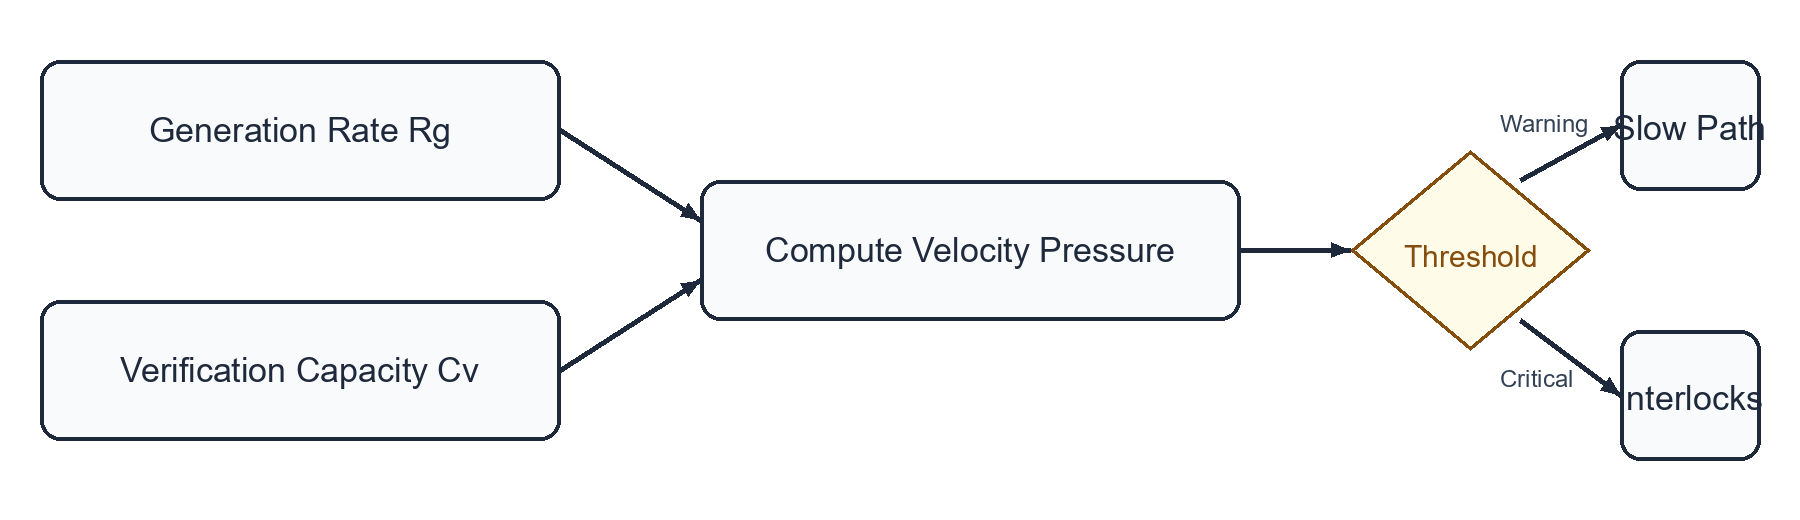
\includegraphics[keepaspectratio,alt={Velocity Pressure Threshold Flow}]{figures/velocity-pressure-threshold.png}}

\begin{center}\rule{0.5\linewidth}{0.5pt}\end{center}

\section{Suggested Citation}\label{suggested-citation}

Overton, K. (2026).\\
\emph{Overton Framework Companion Note v0.1: The Micro-Coercion of
Speed}.\\
CrisisCore-Systems. Zenodo.\\
DOI: Pending (Zenodo will assign upon publication)

\end{document}
